\documentclass{article}

% if you need to pass options to natbib, use, e.g.:
%     \PassOptionsToPackage{numbers, compress}{natbib}
% before loading neurips_2021

% ready for submission
\usepackage[preprint]{neurips_2021}

% to compile a preprint version, e.g., for submission to arXiv, add add the
% [preprint] option:
%     \usepackage[preprint]{neurips_2021}

% to compile a camera-ready version, add the [final] option, e.g.:
%     \usepackage[final]{neurips_2021}

% to avoid loading the natbib package, add option nonatbib:
%    \usepackage[nonatbib]{neurips_2021}

\usepackage[utf8]{inputenc} % allow utf-8 input
\usepackage[T1]{fontenc}    % use 8-bit T1 fonts
\usepackage[colorlinks=true]{hyperref}       % hyperlinks
\usepackage{url}            % simple URL typesetting
\usepackage{booktabs}       % professional-quality tables
\usepackage{amsfonts}       % blackboard math symbols
\usepackage{nicefrac}       % compact symbols for 1/2, etc.
\usepackage{microtype}      % microtypography
\usepackage{xcolor}         % colors
\usepackage{graphicx}
\setcitestyle{numbers,square}

\title{Analyzing the Enron mails}

% The \author macro works with any number of authors. There are two commands
% used to separate the names and addresses of multiple authors: \And and \AND.
%
% Using \And between authors leaves it to LaTeX to determine where to break the
% lines. Using \AND forces a line break at that point. So, if LaTeX puts 3 of 4
% authors names on the first line, and the last on the second line, try using
% \AND instead of \And before the third author name.

\author{%
  Peter Heringer\\
  Matrikelnummer 6109174 \\
  \texttt{peter.heringer@student.uni-tuebingen.de} \\
  \And
  Felix Seidel\\
  Matrikelnummer 5969276 \\
  \texttt{felix.seidel@student.uni-tuebingen.de} \\
}

\begin{document}

\maketitle

\begin{abstract}
  The Enron mail corpus provides real world corporate mail communication data. 
  The corpus contains mails by Enron personell during the phase in which Enron 
  declared bankruptcy. We extract the core working hours of the Enron personell 
  from this dataset. The dataset indicates that Enron performed a migration 
  of their mail systems shortly before the scandal became public, which
  introduces an interesting shift in the mails' time information. However, we
  show that there is no significant change in core working hours over time.
\end{abstract}

\section{Introduction}
After the US energy cooperation Enron declared bankruptcy in 2001
\citep{10.1257/089533003765888403}, law enforcement agencies released enormous
amounts of e-mail communication between Enron employees to the public. This raw
database export was cleaned up as the \emph{Enron Mail Corpus} by
\citet{Klimt2004IntroducingTE}. Today, this dataset contains over 500M mails
from the mailboxes of Enron employees and can be accessed via
\url{https://www.cs.cmu.edu/~enron/}. The e-mails contained in this dataset span
over multiple years, and interestingly, also contain e-mail conversations
throughout 2000 and 2001. As the Enron scandal enrolled during 2001, this period
is interesting in order to check if Enron employees worked differently, i.e.
worked more or less.


\section{Related work}
TODO: Briefly discuss other reports of the mail data.

\section{Analyzing the time data}
For our work we want to investigate whether there was any significant change in
the amount that employees worked during the time that the declared bankruptcy.
This of course is no proof of a direct causal link between these two events, but
makes one at least more plausible.

To analyze this hypothesis one needs to infer the probable working time from the
times the emails were sent. Thus, the first task is to get these timestamps.
As the files contained the headers of the email, the timestamps can be read from
the \texttt{data}-field. To simplify the task only email from sent-folders were
used as this removes automatically many duplicates (emails that are in one
persons sent-folder and in another persons inbox) and mails from automatic
system as well as newsletters. Additionally, from emails that had the same
sender, subject, date and time only one was kept.

\begin{center}
  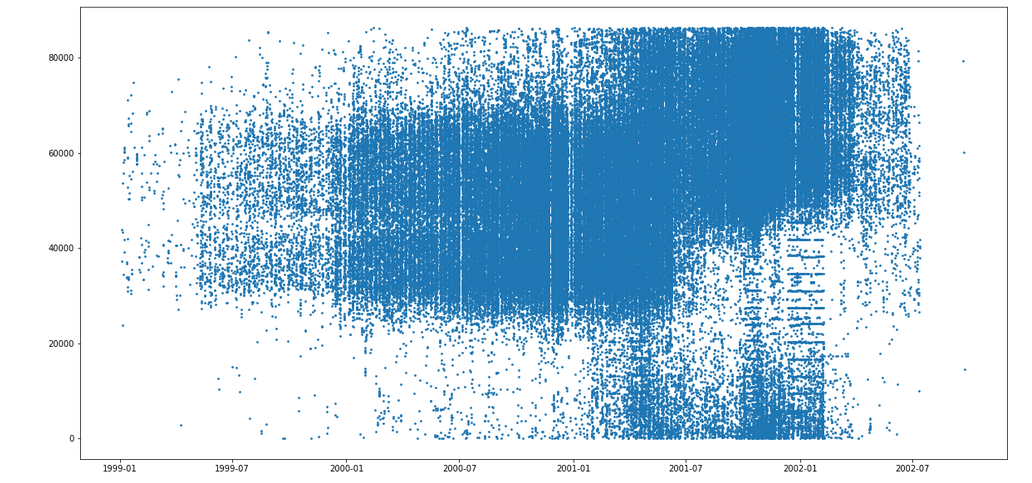
\includegraphics[width=0.7\linewidth]{tmp/plot_all_mail.png}
\end{center}

Depict the different timezones employees appear in (maybe using the boxplot of
all employees and their corresponding mail times), including the timezone used
for the data itself.

Describe the shift that appears in summer 2001
and how we connected that shift to some mail migration. To this end, plot the
mail communication of jeff.dasovich@enron.com over time with all mail data (ie.
the data where only the naive duplicate detection was performed), with the mail
data without duplicates and with the mail data extracted from just the
"sent"-folders.

\begin{center}
  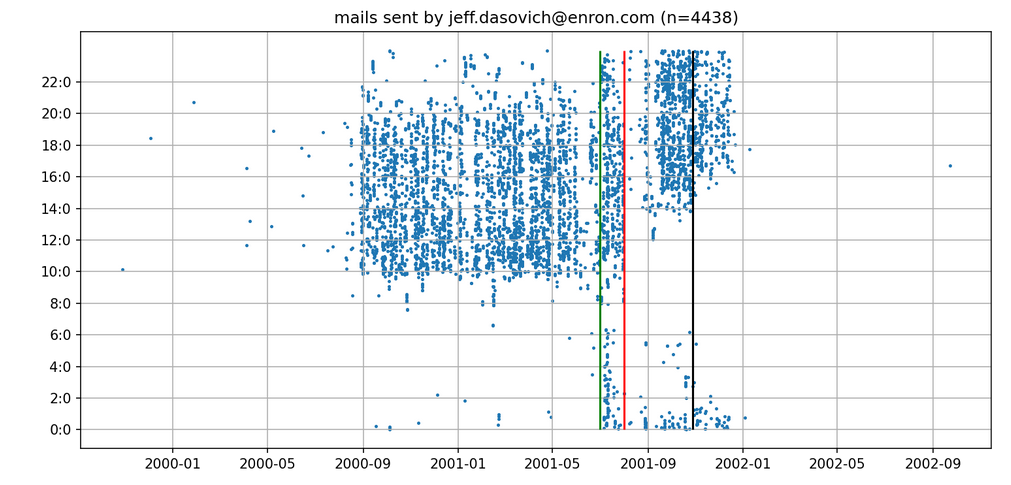
\includegraphics[width=0.7\linewidth]{tmp/plot_jeff_all.png}
\end{center}
\begin{center}
  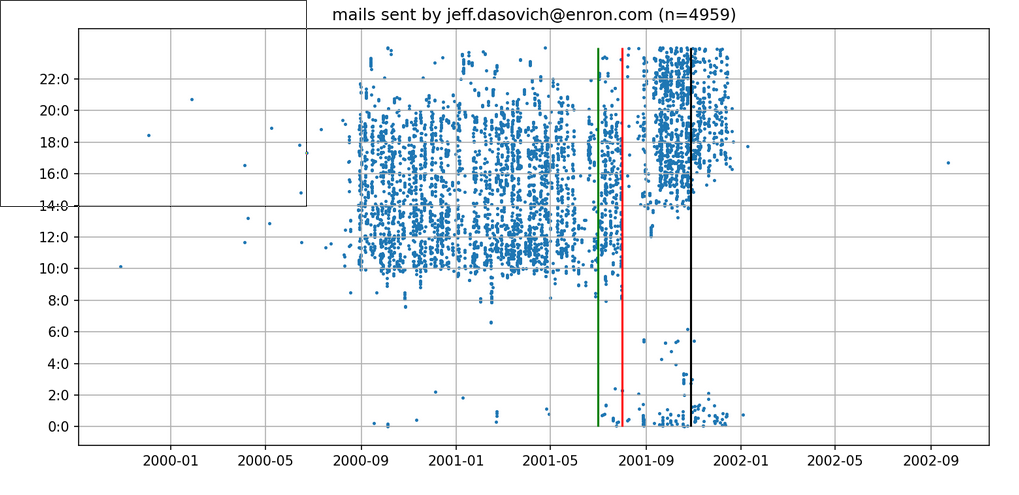
\includegraphics[width=0.7\linewidth]{tmp/plot_jeff_stripped.png}
\end{center}

Describe that this is also visible when making box plots for each month.
\begin{center}
  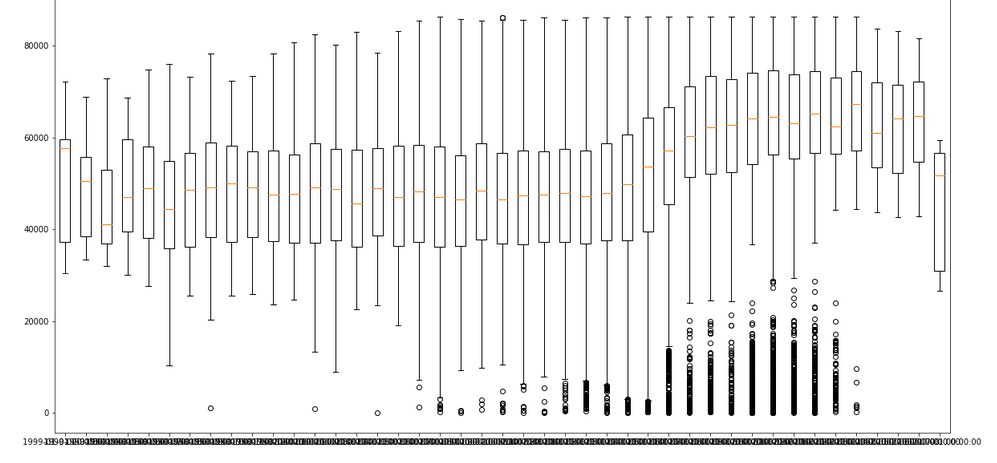
\includegraphics[width=0.7\linewidth]{tmp/boxplot_all.png}
\end{center}

Describe how we calculated the average core working hours for each month based
on that plot. Show how we tested our initial Hypothesis given that data.

\section{Discussion}
Discuss the assumptions that we've made, ie. why we can use the 25/75 quantile,
why we think we can ignore the shift in the mail data, why the assumption of
core working hours is justified.

\section{References}
\bibliographystyle{plainnat}
\bibliography{lib}

\end{document}
